\documentclass[a4paper,12pt]{report}

%%%Преамбула

\usepackage{float}

\usepackage{indentfirst} %Красная строка первого абзаца после заголовка

%структура article следующая:
%part-section-subsection-subsubsection-paragraph-subparagraph

%%%Работа с русским языком
\usepackage{cmap}					% поиск в PDF
%\usepackage{mathtext}			%русские буквы в формулах. КИРИЛЛИЦА НЕ ПРЕДУСМОТРЕНА В ЛАТЕХЕ - лучше отключить
\usepackage[T2A]{fontenc}			% кодировка
\usepackage[utf8]{inputenc}			% кодировка исходного текста
\usepackage[english,russian]{babel}	% локализация и переносы

%%%Шрифты
\usepackage{euscript}		%шрифт Евклид
\usepackage{mathrsfs}		%красивый шрифт

%%%Доп работа с математикой
\usepackage{amsmath,amsfonts,amssymb,amsthm,mathtools} %AMS - корень матана
\usepackage{cases}
\usepackage{icomma} % для отображения запятой как разделителя целой и дробной частей числа

%%%Номера формул
\mathtoolsset{showonlyrefs=true}%Показывать номера только у тех формул, на которые есть \eqref{} в тексте.

%%%Свои команды
\DeclareMathOperator{\sgn}{\mathop{sgn}}
%СИНТАКСИС: \деклейроператор{названиеКоманды}{чтоНужноСделатьКоманде}

%%%Перенос знаков в формулах (по Львовскому) стр 54 мануала
%Т.е. если формула имеет разрыв и переходит на новую строку, то по нормам русского языка арифметический знак должен дублироваться (Латех подчиняется американским нормам, где такого правила нет).
\newcommand*{\hm}[1]{#1\nobreak\discretionary{}%
{\hbox{$\mathsurround=0pt #1$}}{}}

%%%Графика
\usepackage{graphicx} %для \includegraphics{•}
%\usepackage[lofdepth,lotdepth]{subfig}
\graphicspath{{images/}} %теперь пикчи ТеХ будет брать из соответствующей папки в своей домашней папке
\setlength\fboxsep{3pt} %отступ рамки \fbox{} от рисунка
\setlength\fboxrule{1pt} %толщина линий рамки \fbox{}
\usepackage{wrapfig} %обтекание рисунков и таблиц текстом
\usepackage{subcaption}

%%%Таблицы
\usepackage{array,tabularx,tabulary,booktabs} %Доп работа с таблицами
\usepackage{longtable} %длинные таблицы
\usepackage{multirow} %слияние строк в таблице

%%% Программирование
\usepackage{etoolbox} % логические операторы

%%% Страница
%\usepackage{extsizes} % Возможность сделать 14-й шрифт
\usepackage{geometry} % Простой способ задавать поля
	\geometry{top=25mm}
	\geometry{bottom=35mm}
	\geometry{left=35mm}
	\geometry{right=20mm}

%\usepackage{fancyhdr} % Колонтитулы
% 	\pagestyle{fancy}
% 	\renewcommand{\headrulewidth}{0mm}  % Толщина линейки, отчеркивающей верхний колонтитул
 	% \lfoot{Нижний левый}
 	% \rfoot{Нижний правый}
 	% \rhead{Верхний правый}
 	% \chead{Верхний в центре}
 	% \lhead{Верхний левый}
 	% \cfoot{Нижний в центре} % По умолчанию здесь номер страницы

\usepackage{setspace} % Интерлиньяж
\onehalfspacing % Интерлиньяж 1.5
%\doublespacing % Интерлиньяж 2
%\singlespacing % Интерлиньяж 1

\usepackage{lastpage} % Узнать, сколько всего страниц в документе.

\usepackage{soulutf8} % Модификаторы начертания

\usepackage{hyperref}
\usepackage[usenames,dvipsnames,svgnames,table,rgb]{xcolor}
\hypersetup{				% Гиперссылки
    unicode=true,           % русские буквы в раздела PDF
    pdftitle={Заголовок},   % Заголовок
    pdfauthor={Автор},      % Автор
    pdfsubject={Тема},      % Тема
    pdfcreator={Создатель}, % Создатель
    pdfproducer={Производитель}, % Производитель
    pdfkeywords={keyword1} {key2} {key3}, % Ключевые слова
    colorlinks=true,       	% false: ссылки в рамках; true: цветные ссылки
    linkcolor=red,          % внутренние ссылки
    citecolor=green,        % на библиографию
    filecolor=magenta,      % на файлы
    urlcolor=cyan           % на URL
}

%\renewcommand{\familydefault}{\sfdefault} % Начертание шрифта

\usepackage{multicol} % Несколько колонок

\usepackage{enumitem} % Жирные маркеры в begin{enumerate}

%%%Библиография

%\usepackage{cite} % Работа с библиографией (НЕСОВМЕСТИМ С БИБЛАТЕХ)
%\usepackage[superscript]{cite} % Ссылки в верхних индексах
%\usepackage[nocompress]{cite} % 

\usepackage[backend=bibtex, bibencoding=utf8, sorting=ynt, maxcitenames=2, style=numeric]{biblatex}

\usepackage{csquotes} % Еще инструменты для ссылок

\usepackage{multicol} % Несколько колонок
%%% QoL переопределения
\renewcommand{\epsilon}{\varepsilon}

%%% Специфичные знаки с подписями:
% Знак равно с текстом над ним "lambda > 0"
\newcommand\lameq{\mathrel{\overset{\makebox[0pt]{\mbox{\normalfont\tiny\sffamily $\lambda > 0$}}}{=}}}

%%% Теоремы, определения и тд:
% Определение
\theoremstyle{definition}
\newtheorem{definition}{Определение}[section]

% Пример
\theoremstyle{definition}
\newtheorem{example}{Пример}[section]

%\addbibresource{literature.bib}

% После этого part не станет занимать всю страницу
\usepackage{titlesec}
\titleclass{\part}{top}
\titleformat{\part}[display]
{\huge\bfseries\centering}{\partname~\thepart}{0pt}{}
\titlespacing*{\part}{0pt}{40pt}{40pt}

\begin{document}
\begin{titlepage}
\begin{center}
	\textit{федеральное государственное автономное образовательное учреждение \\
		высшего образования}
	\vspace{0.5ex} %вертикальный промежуток = 0.5 от высоты буквы "x" в текущем шрифте.
	
	\textbf{НАЦИОНАЛЬНЫЙ ИССЛЕДОВАТЕЛЬСКИЙ УНИВЕРСИТЕТ \\ <<МОСКОВСКИЙ ФИЗИКО-ТЕХНИЧЕСКИЙ ИНСТИТУТ>>}
\end{center}%выравнивание по центру закончилось

\vspace{13ex}
\begin{flushright}%окружение выравнивает по правому краю текст
	\noindent%убирает красную строку
	\textit{Масленников Никита}\\
	\text{(студент ФАКИ М03-305)}\\
\end{flushright}
\begin{center}
	\vspace{13ex}
	\so{\textbf{Исследовательская работа}}
	\vspace{1ex}
	
	\textbf{\textit{Численное решение задачи Сода и верификация модели на точном решении}}
	
	\vfill %все, что идет после него и до перехода на след. стр. оказалось в самом концу страницы
	Долгопрудный, 2023
\end{center}
\end{titlepage} 

\newpage
 
\hypersetup{linkcolor=black}
\tableofcontents

\newpage
\part*{Основные сокращения и условные обозначения}

\textbf{Сокращения}
\begin{itemize}
\item[НУ] - начальные условия для моделирования задачи или решения уравнений, системы уравнений;
\item[УВ] - ударная волна;
\item[КР] - контактный разрыв;
\item[ВР] - волна разрежения;
\end{itemize}

\textbf{Условные обозначения}
\begin{itemize}
\item [$\rho$] - плотность;
\item [$v$] - скорость;
\item [$E$] - энергия на единицу объема;
\item [$e$] - удельная внутренняя энергия идеального газа;
\item [$\gamma$] - показатель адиабаты;
\end{itemize}
 
\newpage
\part*{Введение}\label{part_intro}

Поставлена задача создать математическую модель численного решения задачи Римана - исследование 1D течения, которое возникает при создании произвольного разрыва в среде. Получившаяся математическая модель проходит верификацию через моделирование задачи Сода и дальнейшей проверкой численного решения с точным.

Программа разбита на 2 части: вычислительная часть реализована на C++, точка входа в программу и обработка результатов написана на Python.

\textbf{Цель работы:}
\begin{enumerate}
\item создание математическую модель численного решения задачи Римана для ударной трубы;
\item верификация модели на задаче Сода;
\item реализация математической модели как отдельный вычислительный модуль для последующей обработки на Python.
\end{enumerate}

Этот документ представляет собой полную информацию о структуре решения задачи Римана для уравнения Эйлера и теоретический материал. Краткое изложение процесса решения находится в Jupyter Notebook.

\newpage

\part{Структура программы}\label{part_structure}

бла бла

\section{Структура решения задачи Римана для уравнения Эйлера}\label{sect_structure}

Уточним задачу Римана: рассмотрим задачу Коши для системы уравнений газовой динамики с разрывом I рода в начальных данных:

\begin{equation}
	\begin{cases}
		\frac{\partial \pmb{q}}{\partial t} + \frac{\partial \pmb{f}}{\partial x} = 0\\
		\pmb{q}(x, 0) =
		\begin{cases}
			\pmb{q}_R,&\text{при}\ x>0\\
			\pmb{q}_L,&\text{при}\ x<0
		\end{cases}
	\end{cases}
\end{equation}
где:
\begin{itemize}
	\item $\pmb{q} = (\rho\quad \rho v\quad E)^T$ - вектор консервативных переменных;
	\item $\pmb{f} = (\rho v\quad \rho v^2 + p\quad (E+p)v)^T$;
	\item $E = \frac{\rho v^2}{2} + \rho e$;
	\item $e = \frac{p}{\rho(\gamma - 1)}$.
\end{itemize}

Структура решения следующая:
\begin{enumerate}
	\item Во входных данных задачи о распаде произвольного разрыва отсутствуют параметры, имеющие размерность длины и времени. Поэтому искомое решение автомодельное;
	\item Класс автомодельных решений для уравнений Эйлера исчерпывается постоянными решениями, в том числе соединенными через разрыв (КР или УВ), а также ВР;
	\item В каждую сторону от разрыва может распространяться не более 1 волны, ударной или разрежения.
\end{enumerate}

\subsection{Возможные конфигурационные решения}\label{sect_configs}

бебра

\subsection{Соотношения для ударных волн}\label{sect_sw}
%sw = shock wave = ударная волна = УВ

бебра

\subsection{Соотношения для волн разрежения}\label{sect_rw}
%rw = rarefaction wave = волна разрежения = ВР

бебра

\subsection{Метод Ньютона}\label{sect_MethNewton}

бебра

\subsection{Распределение физических величин в решении}\label{sect_allSolutions}

бебра

\part{Теория}\label{part_theory}

Рассмотрим уравнение переноса в 1D:

\begin{equation}
	\frac{\partial \pmb{u}}{\partial t} + \frac{\partial \pmb{f}}{\partial x} = 0\\
\end{equation}
где
\begin{itemize}
	\item $f = \lambda u$ - дифференциальный поток.
\end{itemize}

Для численного решения применяется конечно-объемный подход: схема метода конечных объемов. Изменение величины за шаг расчетной ячейки определяется балансом потоков $f$ через грань расчетной ячейки:

\begin{equation}
	\begin{cases}
		\frac{u^{n+1}_{m} - u^{n}_{m}}{\tau} + \frac{1}{h} (f^{n}_{m+\frac{1}{2}}[u^{n}_{m}; u^{n}_{m+1}] - f^{n}_{m-\frac{1}{2}}[u^{n}_{m-1}; u^{n}_{m}])\\
		f^{n}_{m+\frac{1}{2}}[u^{n}_{m}; u^{n}_{m+1}] = f(u_{\text{exact}}(u^{n}_{m}; u^{n}_{m+1})) \ \lameq \ \lambda u^{n}_{m}\\
		f^{n}_{m-\frac{1}{2}}[u^{n}_{m-1}; u^{n}_{m}] = f(u_{\text{exact}}(u^{n}_{m-1}; u^{n}_{m+1})) \ \lameq \ \lambda u^{n}_{m-1}\\
	\end{cases}
\end{equation}
где:
\begin{itemize}
	\item $f^{n}_{*}[u^{n}_{*}; u^{n}_{*}]$ - численный поток, рассчитанный через метод Годунова;
	\item $f(u_{\text{exact}}(u^{n}_{*}; u^{n}_{*}))$ - решение задачи Римана.
\end{itemize}

Существуют различные подходы к построению численного потока $f$: левый уголок. схема Лакса и т.д. Метод Годунова выделяется среди прочих схем: он заключается в расчете потока с использованием точного решения задачи о распаде разрыва.

\begin{definition}
	[Задача о распаде разрыва]
	Задача Коши с кусочно-постоянными данными для задачи гиперболического типа.
\end{definition}

\begin{example}
	[Принцип работы метода Годунова]
	!!! Описать fig\_GodunovMethod и конкретно красную область.
	
	\begin{figure}[h]
		\centering
		
		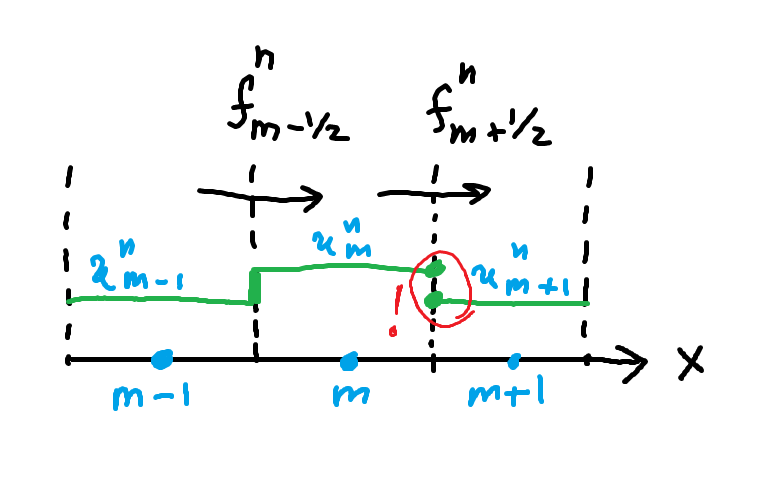
\includegraphics[width=\textwidth]{fig_GodunovMethod}
		\label{fig_GodunovMethod}
	\end{figure}
\end{example}

Каким образом устроено $u_{exact}$ для нелинейных систем уравнений гиперболического типа и конкретно для задачи Эйлера? Ответ на этот вопрос дает краткая теория ниже.

\section{Задача Римана для системы уравнений Эйлера}\label{sect_EulerRiemann}

\begin{equation}
	\begin{cases}
		\frac{\partial \pmb{q}}{\partial t} + \frac{\partial \pmb{f}}{\partial x} = 0\\
		\pmb{q}(x, 0) =
		\begin{cases}
			\pmb{q}_R,&\text{при}\ x>0\\
			\pmb{q}_L,&\text{при}\ x<0
		\end{cases}
	\end{cases}
\end{equation}
где:
\begin{itemize}
	\item $\pmb{q} = (\rho\quad \rho v\quad E)^T$ - вектор консервативных переменных;
	\item $\pmb{f} = (\rho v\quad \rho v^2 + p\quad (E+p)v)^T$;
	\item $E = \frac{\rho v^2}{2} + \rho e$ - энергия на единицу объема;
	\item $e = \frac{p}{\rho(\gamma - 1)}$ - удельная внутренняя энергия идеального газа.
\end{itemize}

\begin{definition}
	[Автомодельное решение]
	Решение, зависящее от $(x, t)$ не произвольным образом, а зависящее от некоторого $\xi = f(x,t)$. Такое решение еще называют \textbf{самоподобным}: решение остается подобным себе с течением времени.
\end{definition}

Решение этой задачи автомодельное - зависит от автомодельной величины $\frac{x}{t}$, т.е. самоподобно течению времени и включает в себя лишь УВ, КР и ВР:

\begin{figure}[H]
	\centering
	
	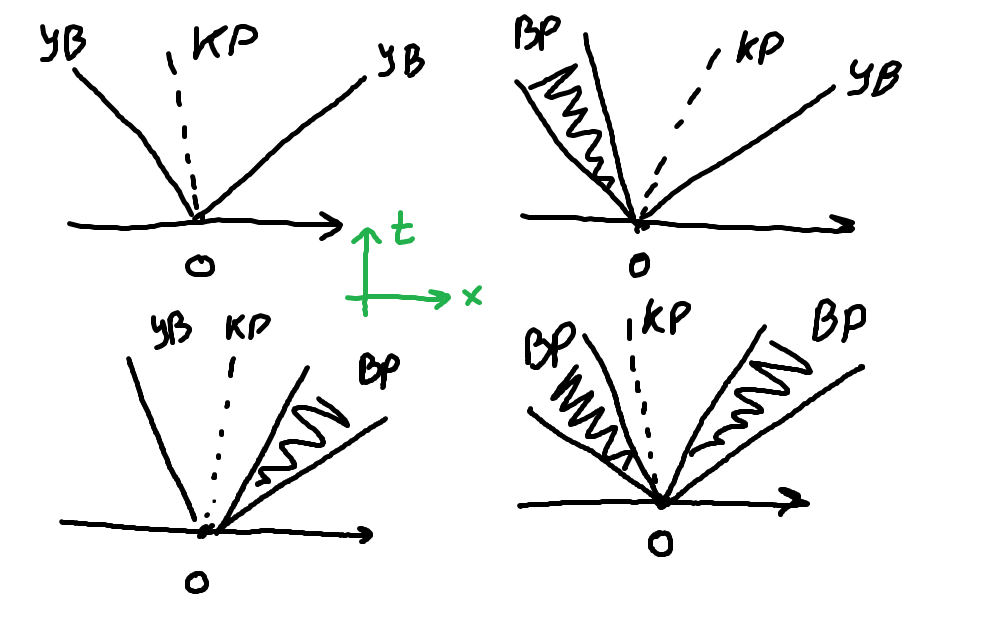
\includegraphics[width=\textwidth]{fig_4configs}
	\caption{Все 4 конфигурации течения}
	\label{fig_4configs}
\end{figure}

\begin{definition}
	[Ударная волна]
	Газодинамический разрыв, который движется внутри среды с постоянной скоростью. Величины $\rho,\ p,\ T,\ v$ испытывают скачок.
\end{definition}

\begin{definition}
	[Волна разрежения]
	Непрерывное решение, ограниченное двумя прямыми линиями. Величины $\rho,\ p,\ T,\ v$ непрерывны.
\end{definition}

\begin{definition}
	[Контактный разрыв]
	Газодинамический разрыв, образование, по разные стороны от которого, среда движется с той же скоростью, что и разрыв. В отличии от УВ, через КР ет протекания вещества и давление с обеих его сторон одинаково. Контактные разрывы также носят название \textbf{тангенциальный разрыв}. Величины $\rho,\ T,\ v$ испытывают скачок.
\end{definition}

\subsection{Одномерные уравнения Эйлера в интегральной форме}\label{sect_EulerIntegralEqs}

Уравнения Эйлера не содержат неразрывных решений, все функции дифференцируемы. Поэтому нужно работать с интегральной формой записи:

\begin{numcases}{}\label{eq: COL_int}
	\oint (pdx - \rho vdt) = 0\\ \label{eq: COMa_int}
	\oint (\rho vdx - [p + \rho v^2]dt) = 0\\ \label{eq: COMo_int}
	\oint (\rho [e + \frac{v^2}{2}]dx - \rho v[e + \frac{v^2}{2} + \frac{p}{\rho}]dt) = 0 \label{eq: COE_int}
\end{numcases}

Течение одномерное и плоское. Вывод интегральной формы (которая в действительности \textbf{первична} дифференциальной) "постулируется"\ и доказывается через систему дифференциальных уравнений и формулу Грина. Рассмотрим разрыв при (x, t) = (0, 0):

\begin{figure}[H]
	\centering
	
	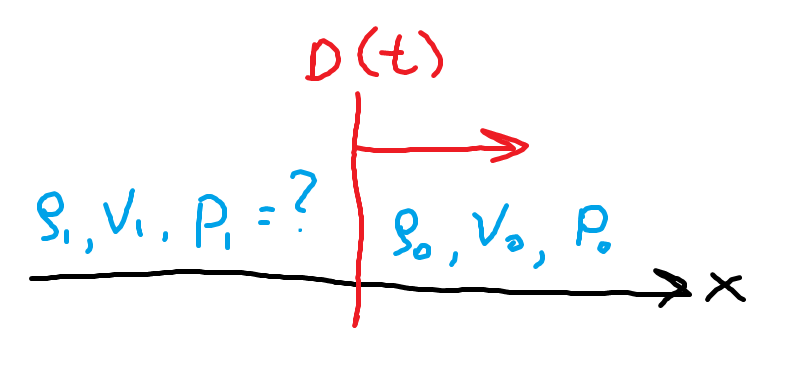
\includegraphics[width=\textwidth]{fig_shock_initial}
	\caption{Момент разрыва}
	\label{fig_shock_initial}
\end{figure}

Рассмотрим пространство (x, t), в котором кривая $PP'$ - траектория разрыва. Тогда смещения на $dx$ задается уравнением:

\begin{equation}\label{eq: COM_int_param}
	dx = D(t)dt
\end{equation}

Выберем контур $AA'B'B$ вокруг $PP'$:

\begin{figure}[H]
	\centering
	
	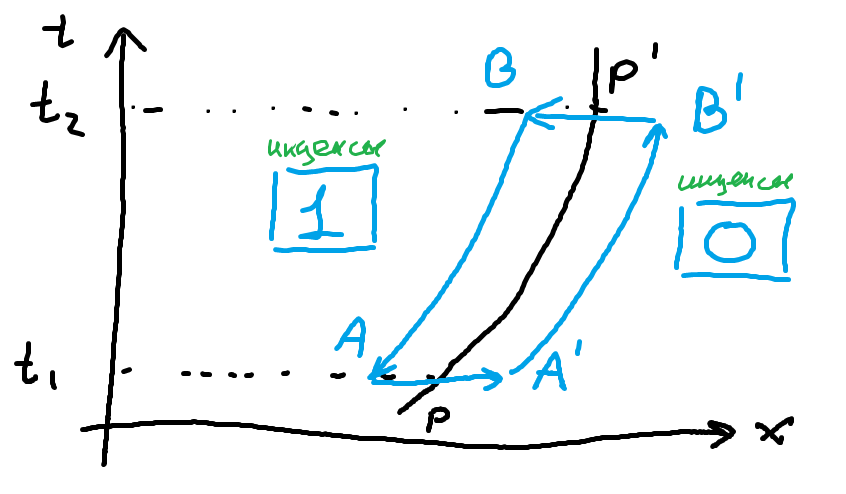
\includegraphics[width=\textwidth]{fig_shock_loop}
	\caption{Схематичное изображение траектории разрыва и контура интегрирования}
	\label{fig_shock_loop}
\end{figure}

Пусть $\Xi = \Xi (\xi)$, где $\xi = \xi(x, t)$ - какой-нибудь интегранд из \refeq{eq: COL_int}. Тогда:

\begin{equation}
	\oint_{AA'B'B} \Xi d\xi = \oint_{AA'} \Xi d\xi + \oint_{A'B'} \Xi d\xi + \oint_{B'B} \Xi d\xi + \oint_{BA} \Xi d\xi = 0
\end{equation}
Далее, устремляем $AA', BB' \rightarrow 0$ и применяем параметризацию \refeq{eq: COM_int_param}:

\begin{equation}
	\oint_{AA'B'B} \Xi d\xi = \oint_{A'B'} \Xi d\xi + \oint_{BA} \Xi d\xi = \int^{t_2}_{t-1} \Xi_{[0]} d\xi + \int^{t_2}_{t_1} \Xi_{[1]} d\xi = 0
\end{equation}
где индексы [0] и [1] означают среды до и после траектории разрыва.

Для \refeq{eq: COMa_int} это будет:

\begin{equation}
	\int^{t_2}_{t_1} (\rho_0 D dt - \rho_0 v_0 dt) + \int^{t_2}_{t_1} (\rho_1 D dt - \rho_1 v_1 dt) = \int^{t_2}_{t_1} (\rho_0 [D-v_0] - \rho_1 [D-v_1]) dt = 0
\end{equation}

Т.к. $t$ выбрано произвольно, то интеграл равен 0 только тогда, когда интегранд равен нулю, а значит $(\rho_0 [D-v_0] - \rho_1 [D-v_1]) = 0$.

\begin{myRemark}
	[Соотношение Ранкина - Гюгонио]
	\begin{equation}
		\rho_0 [D-v_0] = \rho_1 [D-v_1]
	\end{equation}
\end{myRemark}

Если ввести обозначение $[A] = A_1 - A_0$ и ввести $u = v - D$ - скорость газа в системе координат, движущихся вместе с разрывом со скоростью $D$, то \refeq{eq: COL_int} можно переписать как:

\begin{numcases}{} \label{eq: RG_eqs}
	\lbrack \rho u \rbrack = 0\\
	\lbrack \rho u^2 + p \rbrack = 0\\
	\lbrack e + \frac{p}{\rho} + \frac{u^2}{2} \rbrack = 0\\
	\rho u \neq 0
\end{numcases}

По факту доказательство нестрогое. Оно верно, если постулировать законы сохранения с утверждением, что "среда удовлетворяет таким законам".

\subsection{Классификация разрывов}

Путь $m = \rho_0 u_0 = \rho_1 u_1$ - поток массы вещества через разрыв. Тогда существует лишь 2 случая потока:

\begin{itemize}
	\item[a) $m=0$:] Контактные разрывы. Из \refeq{eq: RG_eqs} следует, что \refeq{eq: COMa_int} = 0, а значит:
		\begin{numcases}{}
			v_1 = v_0 = 0\\
			p_1 = p_0\\
			\rho_1 \neq \rho_0
		\end{numcases}
	\item[б) $m \neq 0$:] Ударные волны. Из \refeq{eq: RG_eqs} следует, что \refeq{eq: COMa_int} $\neq$ 0 и:
		\begin{numcases}{}
			v_1 \neq v_0\\
			p_1 \neq p_0\\
			\rho_1 \neq \rho_0
		\end{numcases}
\end{itemize}

\subsection{Адиабата Гюгонио и теорема Цемплена}

Будем исследовать т.н. "Ударные волны разрежения"\ и вопрос их существования. В случае УВ $m \neq 0$ и будем работать с \refeq{eq: COL_int}. При $u = v - D$ и обозначении $\eta = \rho^{-1}$ следует, что:

\begin{numcases}{} \label{eq: SW_adiaGug}
	\frac{\eta_0}{\eta_1} = \frac{u_0}{u_1}\\
	\frac{u_0^2}{\eta_0} - \frac{u_1^2}{\eta_1} = p_1 - p_0\\
	e_1 - e_0 = \frac{u_0^2 - u^2_1}{2} + p_0 \eta_0 - p_1 \eta_1
\end{numcases}

После исключения из рассмотрения скорости, получим следующие формулы. $\eta$ и $p$ понадобится для адиабаты Гюгонио, сама скорость $u$ - для определения скорости скачка относительно газа перед и за УВ:

\begin{numcases}{}
	u_0 = u_1 \frac{\eta_0}{\eta_1}\\
	u_0^2 = \eta_0^2 \frac{p_1 - p_0}{\eta_0 - \eta_1}\\
	u_1 = u_0 \frac{\eta_1}{\eta_0}\\
	u_1^2 = \eta_1^2 \frac{p_1 - p_0}{\eta_0 - \eta_1}
\end{numcases}

\begin{myRemark}
	[Адиабата Гюгонио]
	На диаграмме $(\frac{\eta}{\eta_0}; \frac{p}{p_0})$ описывает все возможные состояния за УВ, куда можно перевести газ, пустив по нему УВ:
	\begin{equation}
		e_1(p_1, \eta_1) - e_0(p_0, \eta_0) = \frac{(p_1 + p_0)(\eta_0 - \eta_1)}{2}
	\end{equation}
\end{myRemark}

Рассмотрим идеальный газ, для которого $e(p, \eta) = \frac{p \eta}{\gamma - 1}$:

\begin{figure}[H]
	\centering
	
	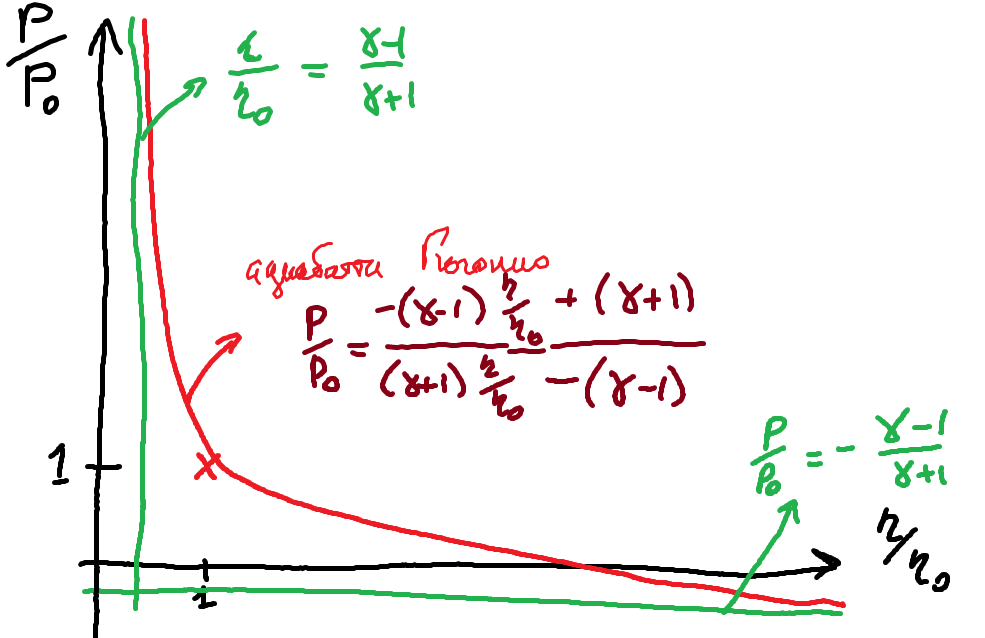
\includegraphics[width=\textwidth]{fig_adiaGug}
	\caption{Адиабата Гюгонио и ее асимптоты}
	\label{fig_adiaGug}
\end{figure}
где:
\begin{itemize}
	\item вертикальная асимптота: не можем считать газ более $\frac{\gamma - 1}{\gamma + 1}$ раз;
	\item горизонтальная асимптота: внезапно отрицательная!? Все потому что законов сохранения энергии \refeq{eq: COL_int} недостаточно для описания всех возможных \textit{физичных} состояний.
\end{itemize}

\begin{theorem}[Теорема Цемплена]
	Не существует УВ разрежения: $\Delta S \geq 0$.
\end{theorem}

То есть теорема Цемплена учитывает Второй закон термодинамики. Получается, что адиабата Гюгонио ложна и не соответствует действительности? На самом деле нет. Переход вещества через ударную волну является \textbf{термодинамически необратимым} процессом, поэтому при прохождении через вещество ударной волны удельная энтропия увеличивается.

Увеличение энтропии означает наличие диссипации (внутри ударной волны, являющейся узкой переходной зоной, существенны, в частности, вязкость и теплопроводность). Это, в частности, приводит к тому, что тело, движущееся в идеальной жидкости с возникновением ударных волн, испытывает силу сопротивления, то есть для такого движения парадокс Д'Аламбера не имеет места.

Ударную адиабату Гюгонио не следует путать с адиабатой Пуассона, описывающей процесс с постоянной энтропией $S$ то есть такие процессы \textbf{термодинамически обратимы}. В отличие от адиабаты Пуассона, для которой $S(p, \eta) = const$ уравнение ударной адиабаты нельзя написать в виде $f(p, \eta) = const$ где $f$ — однозначная функция двух аргументов: адиабаты Гюгонио для заданного вещества составляют двухпараметрическое семейство кривых (каждая кривая определяется заданием как $\eta$ так и $p$ тогда как адиабаты Пуассона — однопараметрическое:

\begin{figure}[H]
	\centering
	
	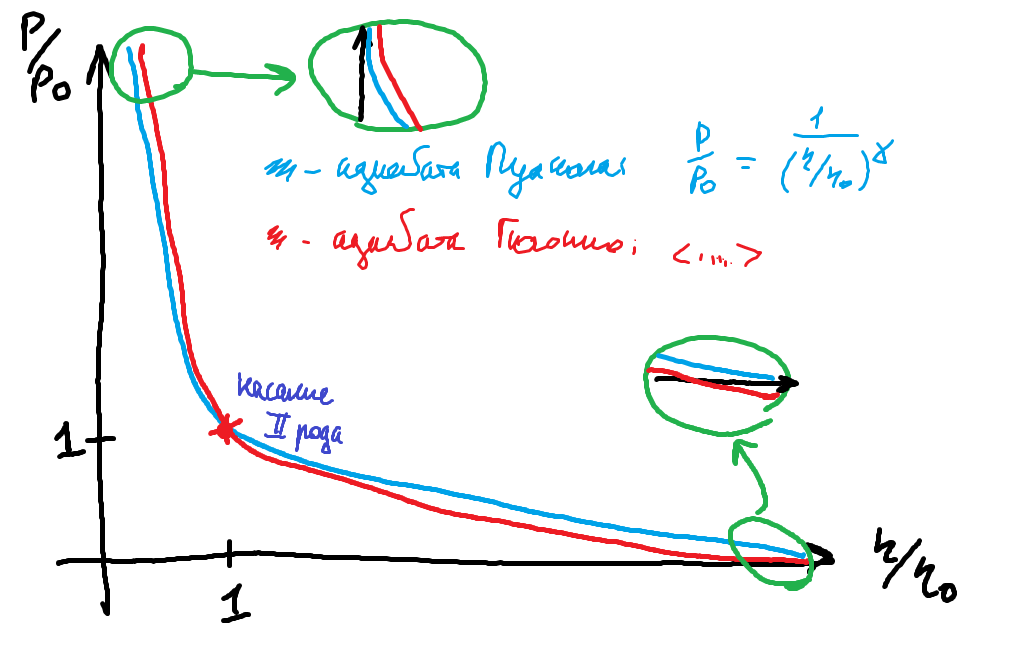
\includegraphics[width=\textwidth]{fig_adiaGugPuas}
	\caption{Адиабаты Гюгонио и Пуассона}
	\label{fig_adiaGugPuas}
\end{figure}

Стоит отметить важный факт: две адиабаты идеально сшиваются по второй производной в точке пересечения. Это знание понадобится для решения задачи Римана (Сода) на (p-v) диаграмме.

\subsection{Звуковая волна}

Из \refeq{eq: SW_adiaGug} мы выражаем $u_0$ и $u_1$. Учитывая, что $c^2 = \gamma p \eta$, вычисляем $\frac{u_i^2}{c_i^2}$:

\begin{numcases}{}
	\frac{u_0^2}{c_0^2} = \frac{(\gamma - 1) + (\gamma + 1) \frac{p_1}{p_0}}{2\gamma}\\
	\frac{u_1^2}{c_1^2} = \frac{(\gamma - 1) + (\gamma + 1) \frac{p_0}{p_1}}{2\gamma}
\end{numcases}

При устремлении $p_1 \rightarrow p_0$ и $\eta_1 \ \rightarrow \eta_0$ и $\frac{u_i^2}{c_i^2} \rightarrow 1$ следует, что УВ бесконечно малой интенсивности распределяется относительно газа со скоростью звука. Т.е. фронт УВ распространяется относительно фона (индекс 0) со сверхзвуковой скоростью, а относительно газа - с дозвуковой:

\begin{figure}[H]
	\centering
	
	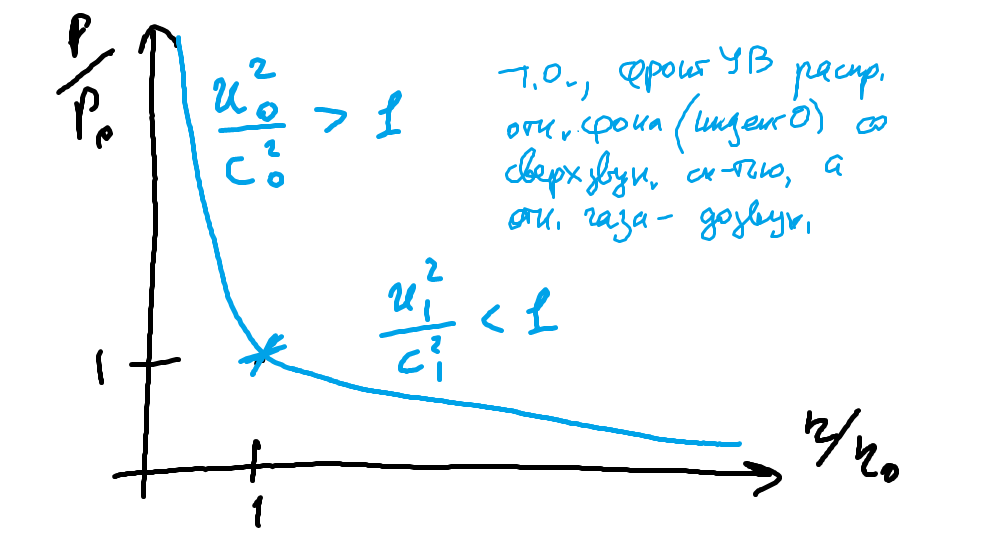
\includegraphics[width=\textwidth]{fig_adiaGugPuas_2}
	\caption{Скорость распространения фронта УВ}
	\label{fig_adiaGugPuas_2}
\end{figure}

\section{Волны Римана}

Будем говорить о характеристическом анализе системы уравнений Эйлера, условий совместности вдоль характеристик и автомодельном решении уравнений Эйлера. Существует две записи системы уравнений Эйлера:
\begin{itemize}
	\item Дивергентная векторная форма:
		\begin{numcases}{}
			\frac{\partial \pmb{q}}{\partial t} + \frac{\partial \pmb{f}}{\partial x} = 0\\
			\pmb{q} = (\rho\quad \rho v\quad E)^T\\
			\pmb{f} = (\rho v\quad \rho v^2 + p\quad (E+p)v)^T\\
			E = \frac{\rho v^2}{2} + \rho e\\
			e = \frac{p}{\rho(\gamma - 1)}
		\end{numcases}
	\item Дивергентная покомпонентная форма:
		\begin{numcases}{} \label{eq: COL_diff}
			\frac{\partial \rho}{\partial t} + \frac{\partial (\rho v)}{\partial x} = 0\\ \label{eq: COMa_diff}
			\frac{\partial (\rho v)}{\partial t} + \frac{\partial (\rho v^2 + p)}{\partial x} = 0\\ \label{eq: COMo_diff}
			\frac{\partial (\rho E)}{\partial t} + \frac{\partial ((\rho E - p)v)}{\partial x} = 0 \label{eq: COE_diff}
		\end{numcases}
\end{itemize}

\subsection{Система уравнений в частных производных 1 порядка гиперболического типа}

Вектор консервативных переменных: $\pmb{q} = (\rho\quad \rho v\quad E)^T$.

Вектор примитивных переменных: $\pmb{U} = \pmb{w} = (\rho\quad v\quad p)^T$

Рассмотрим уравнение:

\begin{equation}
	\frac{\partial \pmb{U}}{\partial t} + \pmb{A}(t, x, \pmb{U}) \frac{\partial \pmb{U}}{\partial x} = \pmb{f}(t, x, \pmb{U})
\end{equation}
где:
\begin{itemize}
	\item $\pmb{U} \in \RealSet^I$
	\item $\pmb{f} \in \RealSet^I$
	\item $\pmb{A} \in \RealSet^{I*I}$
\end{itemize}

\begin{definition}
	[Уравнение гиперболического типа]
	Класс дифференциальных уравнений в частных производных, для которых собственные значения $\lambda_i \in \RealSet$, а собственные вектора образуют базис: $|\Omega_R| \neq 0$.
\end{definition}

Поиск собственных значений и векторов начинается с $\det{\pmb{A} - \lambda \pmb{E}} = 0$, откуда $\lambda_i \in \RealSet, i = \overline{1..I}$. Далее находим соответствующие собственные вектора $\pmb{w}_i \in \RealSet^I$: $(\pmb{A} - \lambda_i \pmb{E}) \pmb{w}_i = 0$.

Мы хотим получить характеристическую покомпонентную форму записи \refeq{eq: COE_diff}. Для этого мы будем почленно дифференцировать слагаемые (как например $\frac{\partial \rho v}{\partial x} = \rho \frac{\partial v}{\partial x} + v \frac{\partial \rho}{\partial x}$) и для \refeq{eq: COE_diff} применим $E = \frac{\rho v^2}{2} + \rho e$ и $e = \frac{p}{\rho(\gamma - 1)}$, как для идеального газа. Получим:

\begin{numcases}{} \label{eq: COL_diff_2}
	\fracPartial[\rho]{t} + \rho \frac{\partial v}{\partial x} + v \frac{\partial \rho}{\partial x} = 0\\
	\fracPartial[v]{t} + v \fracPartial[v]{x} + \frac{1}{\rho} \fracPartial[p]{x} = 0\\
	\fracPartial[p]{t} + \gamma p \fracPartial[v]{x} + v \fracPartial[p]{x} = 0
\end{numcases}

Систему \refeq{eq: COL_diff_2} можно переписать в матричном виде:

\begin{equation} \label{eq: COL_diff_matrix}
	\fracPartial[\pmb{w}]{t} + \pmb{A} \fracPartial[w]{x} = 0
\end{equation}
где:
\begin{itemize}
	\item $\pmb{w} = (\rho\quad v\quad p)^T$ - вектор примитивных переменных;
	\item $\pmb{A} = \begin{pmatrix}
		v & \rho & 0\\
		0 & v & \frac{1}{\rho}\\
		0 & \gamma p & v
	\end{pmatrix}$ - матрица примитивных переменных.
\end{itemize}

Исследование на гиперболичность:

\begin{equation}
	|\pmb{A} - \lambda \pmb{E}| = det
	\begin{pmatrix}
		v - \lambda & \rho & 0\\
		0 & v - \lambda & \frac{1}{\rho}\\
		0 & \gamma p & v - \lambda
	\end{pmatrix} = (v - \lambda)^3 - \frac{\gamma p}{\rho} (v - \lambda) = 0
\end{equation}

Мы введем величину $c = \sqrt{\frac{\gamma p}{\rho}}$ - скорость звука. Решая уравнение выше, приходим к следующим трем собственным значениям:

\begin{numcases}{} \label{eq: eigenVal}
	\lambda_0 = v \in \RealSet\\
	\lambda_1 = v - c \in \RealSet\\
	\lambda_2 = v + c \in \RealSet
\end{numcases}

Собственные значения \refeq{eq: eigenVal} определяют разрыв, три характеристики. $\lambda_0$ соответствует КР:

\begin{figure}[H]
	\centering
	
	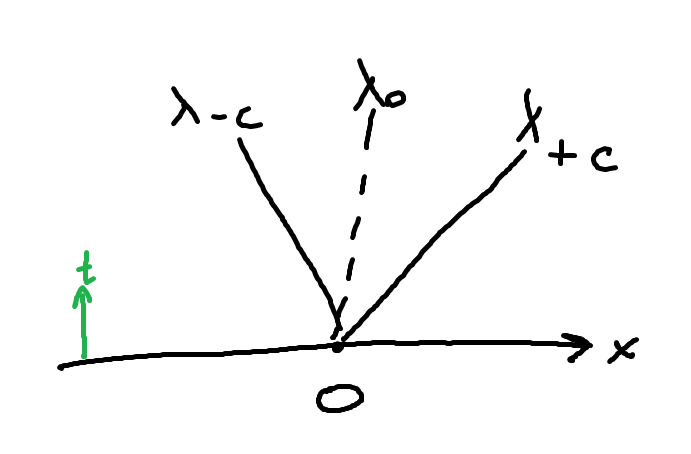
\includegraphics[width=\textwidth]{fig_eigenVals}
	\caption{три характеристики, соответствующие трем собственным значениям}
	\label{fig_eigenVals}
\end{figure}

Далее, собственным значениям \refeq{eq: eigenVal} соответствуют собственные вектора $\pmb{w}_i$. Они образуют матрицы правых и левых собственных векторов:

\begin{definition}
	[Матрица правых собственных векторов]
	Матрица, столбцами которой являются собственные вектора $\pmb{w}_i$:
	
	\begin{equation}
		\pmb{\Omega}_R = \{\pmb{w}_0 \dots \pmb{w}_I\} = 
		\begin{pmatrix}
			1 & \rho & \rho \\
			0 & -c & c \\
			0 & \gamma p & \gamma p
		\end{pmatrix},\quad \det{\pmb{\Omega}_R} = -2\gamma p c \neq 0
	\end{equation}
\end{definition}

\begin{definition}
	[Матрица левых собственных векторов]
	Матрица, обратная $\pmb{\Omega}_R$:
	
	\begin{equation}
		\pmb{\Omega}_L = \pmb{\Omega}_R^{-1} = \frac{1}{\det{\pmb{\Omega}_R}} = 
			\begin{pmatrix}
				-2\gamma p c & 0 & 2 \rho c\\
				0 & \gamma p & -c\\
				0 -\gamma p & -c
			\end{pmatrix}
	\end{equation}
\end{definition}

Если диагональная матрица $\pmb{\Lambda} = diag(v\quad v-c\quad v+c)$, то можем определить матрицу $\pmb{A}$, как:

\[ \pmb{A} = \pmb{\Omega}_R \pmb{\Lambda \Omega}_L \]

\subsection{Условие совместности вдоль характеристик}

Обозначим элементы $\pmb{\Omega}_L$ как $\{\pmb{\Omega}_L\}_{pk}$. Тогда домножим уравнение \refeq{eq: COL_diff_matrix} слева на $\pmb{\Omega}_L$. Ниже представим векторную и покомпонентную запись:

\begin{numcases}{} \label{eq: Euler_syseq_matrix}
	\pmb{\Omega}_L \fracPartial[\pmb{w}]{t} + \pmb{\Lambda} \pmb{\Omega}_L \fracPartial[\pmb{w}]{x} = 0\\
	\sum_{k=1}^{3} \left[ \{\pmb{\Omega}_L\}_{pk} \fracPartial[\pmb{w}_k]{t} \right] + \lambda_p \sum_{k=1}^{3} \left[ \{\pmb{\Omega}_L\}_{pk} \fracPartial[\pmb{w}_k]{x} \right] = 0
\end{numcases}
где $p \in \{0, 1, 2\}$, а $\lambda_p$ определяет направление возмущения.

\subsection{Автомодельное решение уравнения Эйлера и задача Сода}

Ищем решение системы уравнений Эйлера в виде $\pmb{w}(x, t) = \pmb{w}(\xi) = \pmb{w}(\frac{x}{t})$.

\begin{definition}
	[Задача Сода]
	Задача - тест о распаде разрыва со следующими НУ:
	\begin{multicols}{2}
		\begin{itemize}
			\item $p_1 = 1.0$
			\item $\rho_1 = 1.0$
			\item $u_1 = 0.0$
			\item $p_2 = 0.125$
			\item $\rho_2 = 0.1$
			\item $u_2 = 0.0$
		\end{itemize}
	\end{multicols}
\end{definition}

\begin{figure}[H]
	\centering
	
	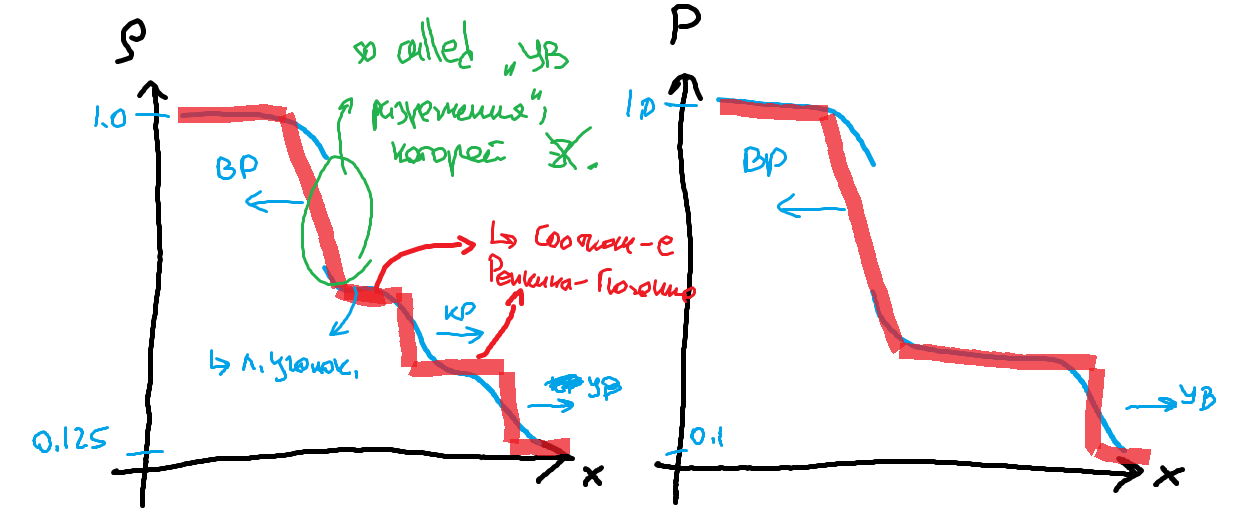
\includegraphics[width=\textwidth]{fig_Soda_rho_p}
	\caption{Точное решение (распространение $\rho$ и $p$) в задаче Сода}
	\label{fig_Soda_rho_p}
\end{figure}

Возвращаясь к поиску решения, найдем производные $\pmb{w}$:

\begin{align}
	\fracPartial[\pmb{w}_k]{x} (x, t) &= \fracPartial[\pmb{w}_k]{\xi} \fracPartial[\xi]{x} = \fracPartial[\pmb{w}_k]{\xi} \frac{1}{t}\\
	\fracPartial[\pmb{w}_k]{t} (x, t) &= \fracPartial[\pmb{w}_k]{\xi} \fracPartial[\xi]{t} = - \fracPartial[\pmb{w}_k]{\xi} \frac{x}{t^2}
\end{align}

После подстановки производных в \refeq{eq: Euler_syseq_matrix} получим:

\begin{equation} \label{eq: automod_vector}
	(\lambda_p - \xi) \sum_{k=1}^{3} \left[ \{\pmb{\Omega}_L\}_{pk} \fracPartial[\pmb{w}_k]{\xi} \right] = 0
\end{equation}
Нам понадобится покомпонентная форма записи:

\begin{numcases}{} \label{eq: automod_scalar_general}
	(\lambda_0 - \xi) \left( 1 \fracPartial[\rho]{\xi} - \frac{\rho}{\gamma p} \fracPartial[p]{\xi} \right) = 0\\ \label{eq: automod_scalar_0}
	(\lambda_1 - \xi) \left( -\frac{1}{2c} \fracPartial[v]{\xi} + \frac{1}{2 \gamma p} \fracPartial[p]{\xi} \right) = 0\\ \label{eq: automod_scalar_1}
	(\lambda_2 - \xi) \left( \frac{1}{2c} \fracPartial[v]{\xi} + \frac{1}{2 \gamma p} \fracPartial[p]{\xi} \right) = 0 \label{eq: automod_scalar_2}
\end{numcases}

\begin{definition}
	[Инвариант Римана]
	Преобразование исходных переменных, в которых система уравнений рассыпалась на совокупность несвязных уравнений переноса.
\end{definition}

Ниже будут исследованы т.н. "левый инвариант Римана"\ и "правый инвариант Римана".
 на основании \refeq{eq: automod_scalar_general}.
\subsection{Левый инвариант Римана}

Нас интересует решение $\xi = \lambda_1$, что соответствует левой-правой ВР:

\begin{numcases}{} \label{eq: LeftRiemann_general}
	\xi = \lambda_1 = v - c\\ \label{eq: LeftRiemann_general_1}
	\fracPartial[\rho]{\xi} - \frac{\rho}{\gamma p} \fracPartial[p]{\xi} = 0\\ \label{eq: LeftRiemann_general_2}
	\frac{1}{2c} \fracPartial[v]{\xi} + \frac{1}{2 \gamma p} \fracPartial[p]{\xi} \label{eq: LeftRiemann_general_3}
\end{numcases}

Вспомним, что нужно добавлять в рассмотрение тот факт, что $\Delta S \geq 0$, у нас это $\fracPartial[S]{\xi} = 0$. Такой процесс называется \textbf{изоэнтропическим}. Для него характерно $\frac{p}{\rho ^ \gamma} = const$: продифференцируем его по $\xi$:

\begin{equation} \label{eq: izoEntr_diff}
	\fracPartial[p]{\xi} - \frac{\gamma p}{\rho} \fracPartial[\rho]{\xi} = 0
\end{equation}

И получается, что \refeq{eq: izoEntr_diff} совпадает с \refeq{eq: LeftRiemann_general_2}! Автомодельное решение соответствует изоэнтропическому течению, где $\fracPartial[S]{\xi} = 0$.

Рассмотрим \refeq{eq: LeftRiemann_general_3}. Учитывая, что $c^2 = \frac{\gamma p}{\rho}$, подставим сюда \refeq{eq: LeftRiemann_general_2}. Тогда:

\begin{equation}
	\fracPartial[c]{\xi} = \frac{c(\gamma - 1)}{2 \rho} \fracPartial[\rho]{\xi}
\end{equation}

\begin{definition}
	[Левый инвариант Римана]
	\begin{equation} \label{eq: LeftRiemann_eq}
		\left( v + \frac{2c}{\gamma - 1} \right)_\xi = (w_L)_\xi = 0
	\end{equation}
\end{definition}

\begin{definition}
	[Левая волна]
	Волна называется \textbf{"левой"}, если поток массы через нее направлен слева-направо:
	\[ \rho (v - \xi) > 0\]
\end{definition}

Т. е. изменение левого инварианта Римана в поле рассматриваемого течения равно нулю. Тогда автомодельное решение в уравнении Эйлера соответствует такому типу течения, в котором левая волна Римана - ВР. она удовлетворяет:

\begin{numcases}{}
	v - c = \frac{x}{t}\\
	S = \frac{p}{\rho^\gamma = const}\\
	w_L = v + \frac{2c}{\gamma - 1} = const
\end{numcases}

\begin{figure}[H]
	\centering
	
	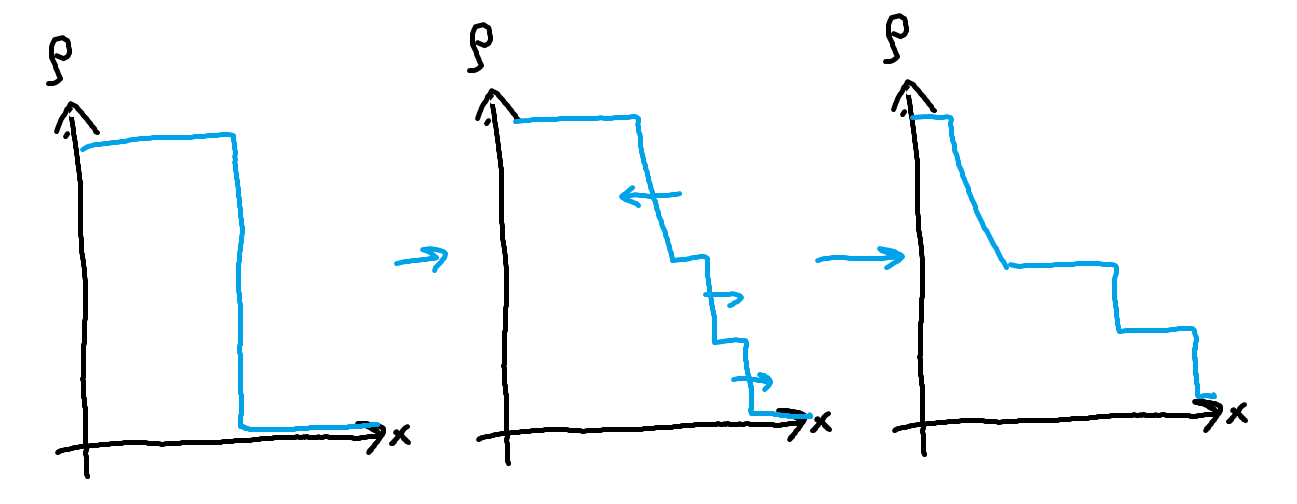
\includegraphics[width=\textwidth]{fig_LeftRiemann_graph}
	\caption{Тип течения, в котором левая волна Римана - ВР}
	\label{fig_LeftRiemann_graph}
\end{figure}

\subsection{Правый инвариант Римана}

Нас интересует решение $\xi = \lambda_2$, что соответствует левой-правой ВР:

\begin{numcases}{} \label{eq: RightRiemann_general}
	\xi = \lambda_1 = v - c\\ \label{eq: RightRiemann_general_1}
	\fracPartial[\rho]{\xi} - \frac{\rho}{\gamma p} \fracPartial[p]{\xi} = 0\\ \label{eq: RightRiemann_general_2}
	\frac{1}{2c} \fracPartial[v]{\xi} + \frac{1}{2 \gamma p} \fracPartial[p]{\xi} \label{eq: RightRiemann_general_3}
\end{numcases}

Проделывая те же действия, что и для левого инварианта Римана, получим следующую систему уравнений:

\begin{numcases}{}
	\xi = v + c\\
	\fracPartial[S]{\xi} = 0\\
	w_R = v - \frac{2c}{\gamma - 1} = const
\end{numcases}

\begin{definition}
	[Правая волна]
	Волна называется \textbf{"правой"}, если поток массы через нее направлен справа-налево:
	\[ \rho (v - \xi) < 0\]
\end{definition}

\begin{figure}[H]
	\centering
	
	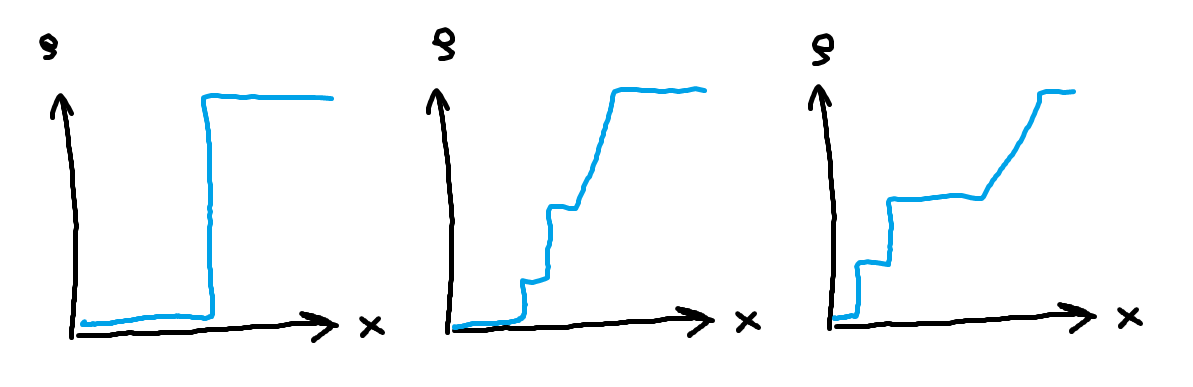
\includegraphics[width=\textwidth]{fig_RightRiemann_graph}
	\caption{Тип течения, в котором правая волна Римана - ВР}
	\label{fig_RightRiemann_graph}
\end{figure}

\begin{definition}
	[Правый инвариант Римана]
	\begin{equation} \label{eq: RightRiemann_eq}
		\left( v - \frac{2c}{\gamma - 1} \right)_\xi = (w_R)_\xi = 0
	\end{equation}
\end{definition}

%\printbibliography
\end{document}
